\subsection{System Implementation}
The implemented system for this thesis is kept simple with one device on each computation layer. The esp32 connected to a button and light is the IoT device makes up the IoT layer, the RPi the edge layer and the VPS the cloud part. This is shown in \cref{fig:actualSetup}.
\begin{figure}
    \centering
    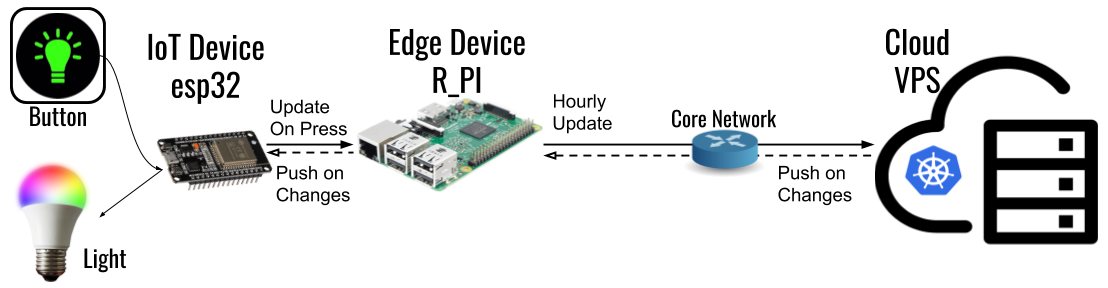
\includegraphics[width=\textwidth]{figures/actualSetup.png}
    \caption{The implemented system.}
    \label{fig:actualSetup}
\end{figure}
On the edge we have little latency 



\Cref{sec:desiredSystem} presented the ideal system with the resources provided for this thesis. Following the classification via the MoSCoW method major and minor changes to the ideal setup had to made as technology and time didn't not allow for a full implementation. \cref{fig:actualImplementationSetup} shows the actual implementation.
\begin{figure}
    \centering
    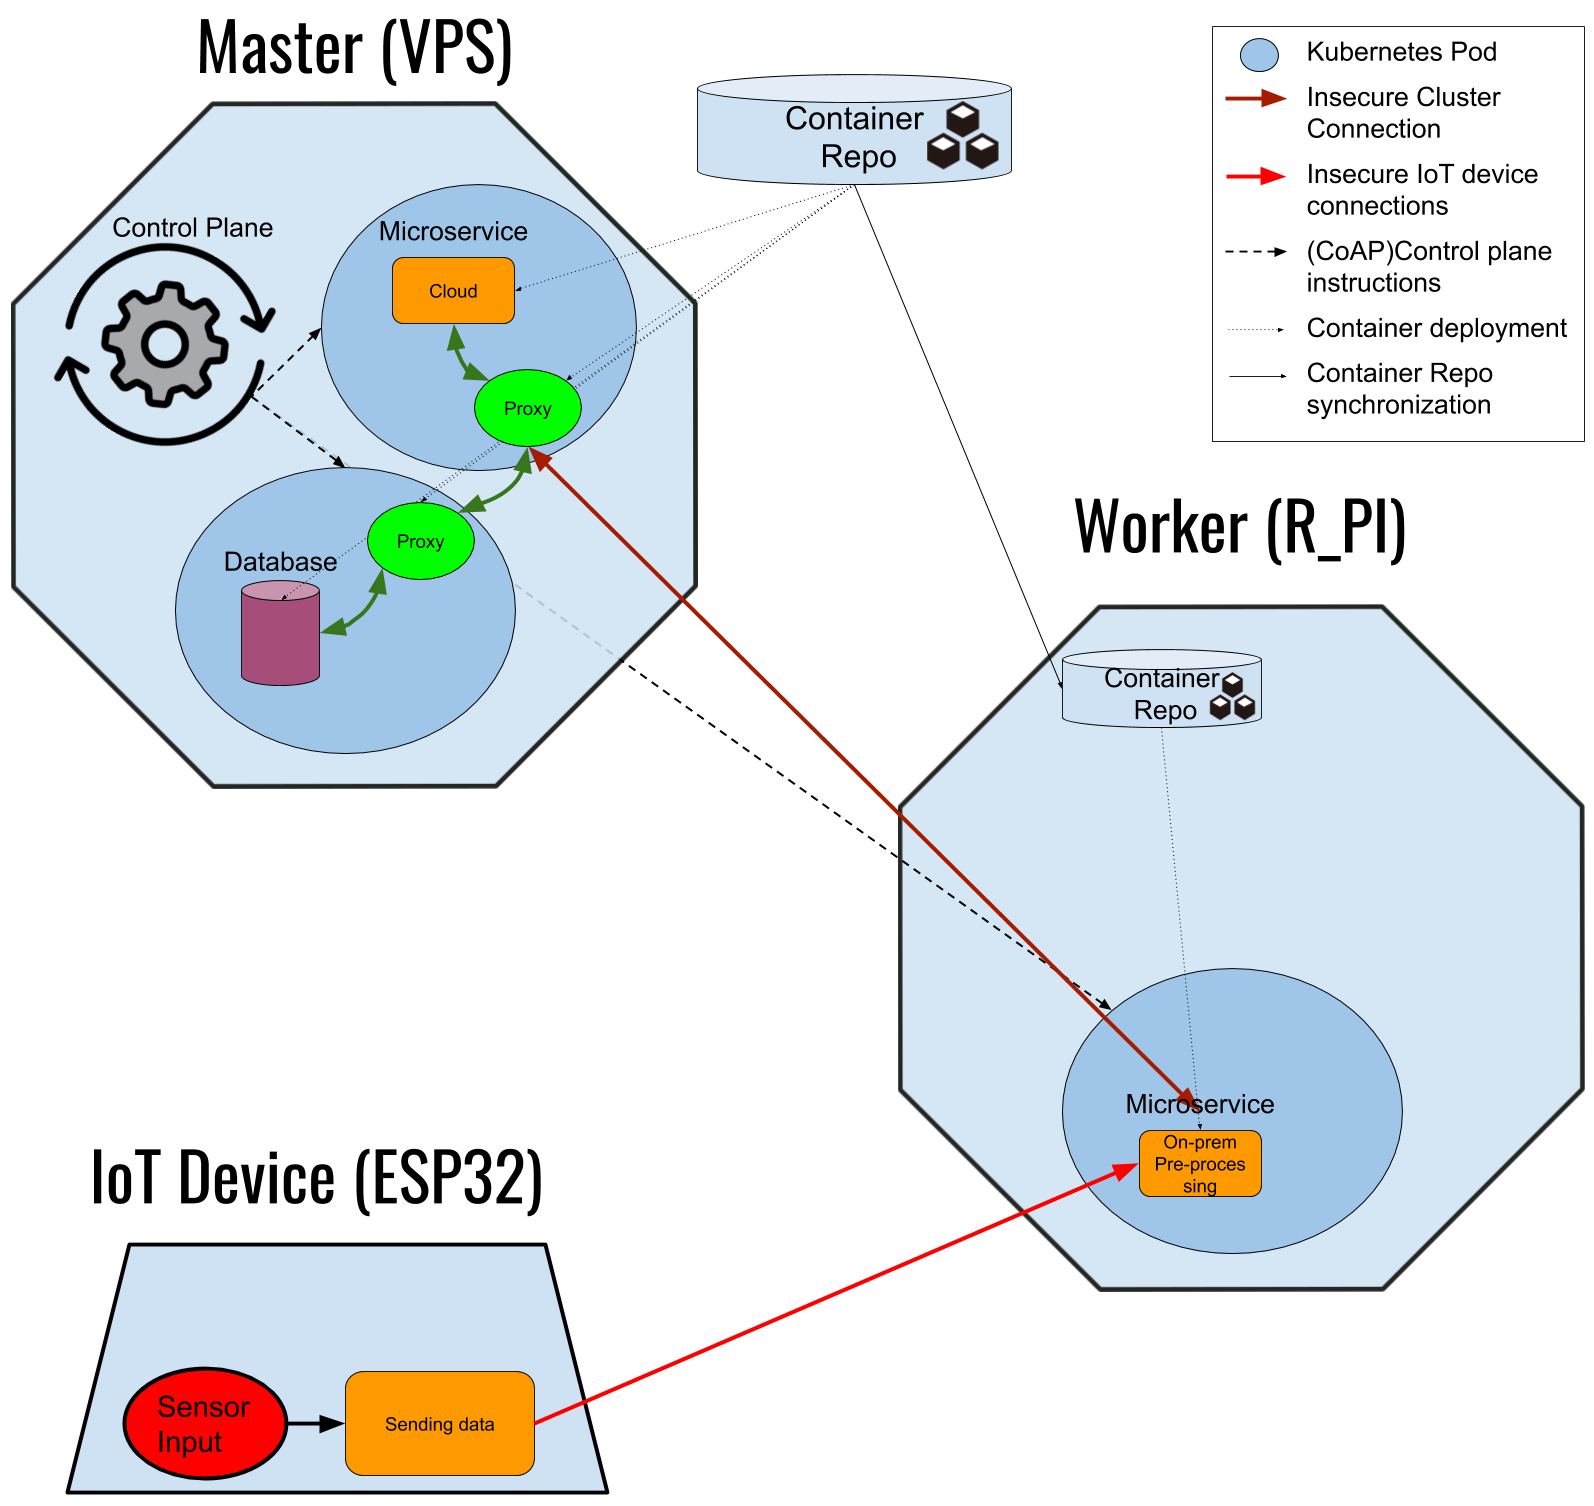
\includegraphics[width=\textwidth]{figures/actualImplementationSetup.png}
    \caption{The actual system architecture of the implementation.}
    \label{fig:actualImplementationSetup}
\end{figure}
The cloud part is unchanged from the desired setup, on the edge part however adoptions had to be made. The Istio envoy proxy does not compile for the ARM architecture yet, so the traffic will not be encrypted. It is true that encryption could still be made, but that would create the difficulties of handling certificates into the administrators hands. It also makes it impossible to reroute network traffic from the application to another destination. Istio enables a whole set of traffic management, which is not available if its proxy is not able to run inside the pod.\\
The connection from the 